\documentclass[../../../../main.tex]{subfiles}
\begin{document}
\section*{京都大学 1987年 前期}
\begin{center}
100/120分
\vspace{1ex}

\begin{tabular}{|c|l|c|c|c|l|}
\hline
& & 計 & 思 & 総 & \\ \hline
[1] & 関数 & A & A & A & 20 \\ \hline
[2] & & & & & \\ \hline
[3] & 多変数 & C & B & B & 20 \\ \hline
[4] & 関数 & B & B & B & 20 \\ \hline
[5] & 多変数 $*$ & C & B & B & 20 \\ \hline
[6] & 確率 & C & B & B & \textcircled{未} \\ \hline
\end{tabular}
\end{center}

\subsection*{第1問}
[解]
\begin{equation*}
\begin{cases}
f(x) = (ax+b)h(x) + cx + a^2-a \\
g(x) = (ax-b^2)h(x) + (a-1)x + c^2
\end{cases} \quad (a \neq 0)
\end{equation*}

より、
\begin{align*}
f(x)\text{が}h(x)\text{で割り切れる} &\iff \begin{cases} c=0 \\ a(a-1)=0 \end{cases} \quad \cdots \text{\textcircled{A}} \\
g(x)\text{が \quad \ \ \ \ \ \ \ \ \ \ \ \ \ \ \ \ \ } &\iff \begin{cases} a-1=0 \\ c^2=0 \end{cases}
\end{align*}

だから、\textcircled{A}の時、$a \neq 0$から$c=0 \land a=1$で、たしかに$g(x)$は$h(x)$で割り切れる。
一方、\textcircled{A}でないとき つまり $c \neq 0$ or $a \neq 1$ の時、
たしかに$g(x)$も$h(x)$では割り切れない。

よって示された。$\blacksquare$

\subsection*{第2問}

\subsection*{第3問}
[解] $c = \cos\theta \ (-1 \le c \le 1)$ とおくと
\begin{equation*}
(\text{与式}) \iff a(2c^2-1) + bc - 1 < 0 \quad \cdots \text{\textcircled{1}}
\end{equation*}
\textcircled{1}の左辺$f(c)$とおき、$f(c)<0$ となる条件をしらべる。\\
$f'(c) = 2ac+b$ である。

$1^\circ \ a=0$の時、$f(c)$は高々一次関数だから
\begin{align*}
&f(1) < 0 \land f(-1) < 0 \\
\iff & -1 < b < 1
\end{align*}

$2^\circ \ a>0$の時\\
$f(c)$の軸 $c = -\frac{b}{4a}$ によらず、$f(c)$は $c = \pm 1$で最大で
\begin{align*}
&f(1) < 0 \land f(-1) < 0 \\
\iff & a+b-1 < 0 \land a-b-1 < 0
\end{align*}

$3^\circ \ a<0$の時
\begin{align*}
&\text{\textcircled{ア}} \ -1 \le -\frac{b}{4a} \le 1 \text{の時} \quad f(-\frac{b}{4a}) < 0 \iff \frac{(a+\frac{1}{2})^2}{1/4} + \frac{b^2}{1} < 1 \quad \cdots \text{A} \\
&\text{\textcircled{イ}} \ -\frac{b}{4a} \le -1 \text{の時} \quad f(-1) < 0 \\
&\text{\textcircled{ウ}} \ -\frac{b}{4a} \ge 1 \text{の時} \quad f(1) < 0
\end{align*}

以上まとめて
\begin{itemize}
\item $a \ge 0 \land a-1 < b < a+1$
\item $4a \le b \le -4a \land a < 0 \land \frac{(a+\frac{1}{2})^2}{1/4} + \frac{b^2}{2} < 1$
\item $4a \ge b \land a < 0 \land a-1 < b$
\item $-4a \le b \land a < 0 \land b < -a+1$
\end{itemize}

これを図示して下図(境界含まず)

\begin{center}
\begin{tikzpicture}[scale=1.5]
\draw[->] (-2,0) -- (1.5,0) node[right] {$a$};
\draw[->] (0,-2.5) -- (0,2.5) node[above] {$b$};
\draw[dashed] (-1, -2) -- (0.5, 2.5) node[right] {$b=4a$};
\draw[dashed] (-1, 2) -- (0.5, -2.5) node[right] {$b=-4a$};
\draw (-1.5, -0.5) -- (0,1) node[right] {$b=a+1$};
\draw (-1.5, 0.5) -- (0,-1) node[right] {$b=-a-1$};
\draw (0,1) -- (1,2) node[right] {};
\draw (0,-1) -- (1,-2) node[right] {};
\draw[domain=-1:0, smooth, variable=\a, blue] plot ({\a}, {sqrt(2*(1 - 4*(\a+0.5)^2))});
\draw[domain=-1:0, smooth, variable=\a, blue] plot ({\a}, {-sqrt(2*(1 - 4*(\a+0.5)^2))});
\node at (-0.5, 0) [below] {$-\frac{1}{2}$};
\node at (-1, 0) [below left] {$-1$};
\node at (0, 0) [below right] {$O$};
\node at (-0.33, 0) [below] {$-\frac{1}{3}$};
\node[blue] at (1.5, 1) {[本時のミス]};
\node[blue] at (1.5, 0.5) {$\cdot$ 計算ミス};
\node[blue] at (1.5, 0) {$\cdot$ 軸についての勘違い};
\node at (-1, 1.5) {$\frac{(a+1/2)^2}{1/4} + \frac{b^2}{2} = 1$};
\node at (2.5, 2) {$4(a+1/2)^2 + \frac{b^2}{2} = 1, \ b = \pm (a-1) \text{ を連立すると}$};
\node at (2.5, 1.5) {$4(a+1/2)^2 + \frac{1}{2}(a^2-2a+1) = 1$};
\node at (2.5, 1) {$9a^2+6a+1 = 0 \qquad \therefore a=-\frac{1}{3}$};
\node at (2.5, 0.5) {$\text{から接している}$};
\end{tikzpicture}
\end{center}

\subsection*{第4問}
[解]
(1) $f'(x) = 3x^2+2ax+b$ から、3次関数では接点と接線が一対一対応するので、$f'(x)=m$となる$x$の数にひとしい。\\
$f'(x)-m=0 \ \cdots$ \textcircled{1} の判別式$D$として
\begin{align*}
& \begin{cases}
D>0 \iff a^2-3(b-m)>0 & \text{の時 } 2\text{コ} \\
D=0 \iff a^2-3(b-m)=0 & \qquad 1\text{コ} \\
D<0 \iff a^2-3(b-m)<0 & \qquad 0\text{コ}
\end{cases} \quad \text{\#\ \ }
\end{align*}

(2) $P_1, P_2$の$x$座標 $\alpha, \beta$ とおく ($\alpha < \beta$としてよい)。と、これらは\textcircled{1}の2実数解である。\\
$l_1 : y=l_1(x), l_2 : y=l_2(x)$; $Q_1, Q_2$の$x$座標$q_1, q_2$として
\begin{align*}
f(x) - l_1(x) &= (x-\alpha)^2 (x-q_1) \quad \cdots \text{\textcircled{2}} \\
f(x) - l_2(x) &= (x-\beta)^2 (x-q_2) \quad \cdots \text{\textcircled{3}}
\end{align*}
$f(x)$は3次、$l_1(x), l_2(x)$は1次だから、2次の係数を比較して
\begin{align*}
& a = -2\alpha - q_1 = -2\beta - q_2 \\
& \text{（$a = -\frac{3}{2}(\alpha+\beta)$ だから辺々たして代入）} \\
& -3(\alpha+\beta) = -2(\alpha+\beta) - (q_1+q_2) \\
& \alpha+\beta = q_1+q_2 \\
& \therefore |\alpha-q_1| = |q_2-\beta|
\end{align*}
だから、$P_1, Q_1$の$x$座標の差と $P_2, Q_2$のそれが等しく、さらに$P_1Q_1, P_2Q_2$の傾きも等しいので、$\overline{P_1Q_1} = \overline{P_2Q_2}$ \quad $\blacksquare$

\vspace{1ex}
\noindent
[解2] [例の対称性を用いる]

$P_1(x_1, f(x_1)), P_2(x_2, f(x_2))$ の中点$M(p,q)$とすると
\begin{align*}
\begin{cases}
p = \frac{x_1+x_2}{2} \\
q = \frac{f(x_1)+f(x_2)}{2}
\end{cases}
\end{align*}
解と係数の関係から
\begin{align*}
q &= \frac{1}{2}(x_1^3+x_2^3) + \frac{a}{2}(x_1^2+x_2^2) + \frac{b}{2}(x_1+x_2) + c \\
&= \frac{2}{27}a^3 - \frac{ab}{3} + c \\
f(p) &= \left(\frac{x_1+x_2}{2}\right)^3 + \frac{a}{2}\left(\frac{x_1+x_2}{2}\right)^2 + b\left(\frac{x_1+x_2}{2}\right) + c = \frac{2}{27}a^3 - \frac{ab}{3} + c = q
\end{align*}
より、$M$は曲線上の点。次に$M$が原点になるように$f(x)$を平行移動すると
\begin{align*}
Y = X^3 + \left(b-\frac{a^2}{3}\right)X
\end{align*}
これは奇関数だから原点対称。よって$M$に関する対称性により$P_2, Q_2$を$P_1, Q_1$に重ねあわせることができるから\\
$\overline{P_1Q_1} = \overline{P_2Q_2}$ \quad $\blacksquare$

\begin{center}
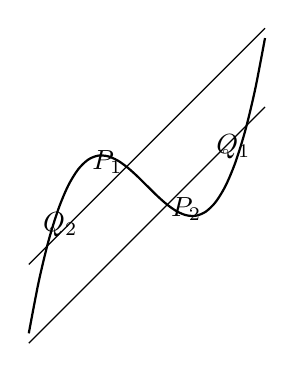
\begin{tikzpicture}
\draw[thick, domain=-1.5:1.5, smooth, variable=\x] plot ({\x}, {\x^3 - \x});
\node at (1.1, 0.5) {$Q_1$};
\node at (-1.1, -0.5) {$Q_2$};
\node at (-0.5, 0.3) {$P_1$};
\node at (0.5, -0.3) {$P_2$};
\draw (-1.5, -1) -- (1.5, 2);
\draw (-1.5, -2) -- (1.5, 1);
\end{tikzpicture}
\end{center}


\subsection*{第5問}
[解] (1) $T: ax+y+z+a-2=0$ とする。$T$の法線ベクトルの1つに$\vec{n} = \begin{pmatrix} a \\ 1 \\ 1 \end{pmatrix}$がある。題意の点$P$とすると、$OP \perp T$ だから、$k \in \mathbb{R}$として
\begin{equation*}
\overrightarrow{OP} = k\vec{n} \quad \cdots \text{\textcircled{1}}
\end{equation*}
とかける。これが$T$上の点だから、
\begin{align*}
a(ka) + (k) + (k) + a-2 &= 0 \qquad \therefore k = \frac{2-a}{a^2+2}
\end{align*}
となって \textcircled{1}から
\begin{align*}
P\left( \frac{(2-a)a}{a^2+2}, \frac{2-a}{a^2+2}, \frac{2-a}{a^2+2} \right) \quad \text{\#\ \ }
\end{align*}

(2) 平面と点のキョリ公式から
\begin{align*}
|OP| &= \frac{|a-2|}{\sqrt{a^2+1+1}} = \frac{|a-2|}{\sqrt{a^2+2}} \quad (\equiv f(a) \text{とする})
\end{align*}
である。まず $\left\{ f(a) \right\}^2 = \frac{(a-2)^2}{a^2+2}$ の値域をもとめる。
\begin{align*}
\left\{ f(a)^2 \right\}' &= \frac{2(a-2)(a^2+2) - 2a(a-2)^2}{(a^2+2)^2} = \frac{2(a-2)(2a+2)}{(a^2+2)^2}
\end{align*}
から増減表をうる。

\begin{center}
\begin{tabular}{|c|c|c|c|c|c|}
\hline
$a$ & $\cdots$ & $-1$ & $\cdots$ & $2$ & $\cdots$ \\ \hline
$f'$ & $+$ & $0$ & $-$ & $0$ & $+$ \\ \hline
$f^2$ & $\nearrow$ & $3$ & $\searrow$ & $0$ & $\nearrow$ \\ \hline
\end{tabular}
\end{center}

したがって、$0 \le f(a)$とあわせて、$\max f(a) = \sqrt{3}$である。$V(a) \text{が}\min \iff f(a) \text{が}\max$ だから\\
$a=-1$の時、
\begin{align*}
\min V(a) &= \pi \int_{\sqrt{3}}^3 (9-x^2)dx = \pi \left[ 9x - \frac{1}{3}x^3 \right]_{\sqrt{3}}^3 = \pi (18 - 8\sqrt{3}) \quad \text{\#\ \ }
\end{align*}
をとる。

\subsection*{第6問}
[解] 赤玉R, 白玉Wと表す。人が死かえてえらぶかは確率1/2で同様にたからしい。\\
(1)
\begin{center}
\begin{tabular}{|c|c|c|c|l|}
\hline
& A & B & C & \\ \hline
(R,W) & (1,1) & (1,1) & (1,1) & $F_0$ \\ \hline
(R,W) & (1,1) & (0,2) & (2,0) & $F_1$ \\ \hline
(R,W) & (2,0) & (0,2) & (1,1) & $F_2$ \\ \hline
(R,W) & (1,1) & (2,0) & (0,2) & $F_3$ \\ \hline
(R,W) & (0,2) & (2,0) & (1,1) & $F_4$ \\ \hline
(R,W) & (0,2) & (1,1) & (2,0) & $F_5$ \\ \hline
(R,W) & (2,0) & (1,1) & (0,2) & $F_6$ \\ \hline
\end{tabular}
\end{center}

(2)
\begin{align*}
\begin{cases}
P_{00} = \frac{1}{4} \\
P_{0k} = \frac{1}{8} \ (k=1,2,\cdots,6)
\end{cases}
\end{align*}
\begin{align*}
\begin{cases}
P_{1k} = 0 \quad (k=1,3,4,5,6) \\
P_{10} = P_{12} = \frac{1}{2}
\end{cases}
\end{align*}
\begin{align*}
\begin{cases}
P_{2k} = 0 \ (k=1,2,3,4,5) \\
P_{20} = P_{26} = \frac{1}{2}
\end{cases}
\end{align*}
\begin{align*}
\begin{cases}
P_{3k} = 0 \ (k=1,2,3,5,6) \\
P_{30} = P_{34} = \frac{1}{2}
\end{cases}
\end{align*}
\begin{align*}
\begin{cases}
P_{4k} = 0 \ (k=1,3,4,5,6) \\
P_{40} = P_{45} = \frac{1}{2}
\end{cases}
\end{align*}
\begin{align*}
\begin{cases}
P_{5k} = 0 \ (k=2,3,4,5,6) \\
P_{50} = P_{51} = \frac{1}{2}
\end{cases}
\end{align*}
\begin{align*}
\begin{cases}
P_{6k} = 0 \\
P_{60} = P_{63} = \frac{1}{2}
\end{cases}
\end{align*}

(3) (1)から
\begin{align*}
\begin{cases}
q_{n+1} = \frac{1}{4}q_n + \frac{1}{2}(1-q_n) \\
\qquad = -\frac{1}{4}q_n + \frac{1}{2} \\
q_0 = 1
\end{cases}
\end{align*}
だから、等比数列の公式から
\begin{align*}
q_n &= \left(-\frac{1}{4}\right)^n \left(1 - \frac{2}{5}\right) + \frac{2}{5} \\
&= \frac{3}{5}\left(-\frac{1}{4}\right)^n + \frac{2}{5} \quad \text{\#\ \ }
\end{align*}

\end{document}
